\documentclass[prl,onecolumn,lengthcheck]{revtex4-2}

\usepackage{amssymb, amsmath, amsthm, amstext, amsfonts, amsopn, amscd}
\usepackage{dsfont}% provides \mathds{1} for the \1 macro

\usepackage{color}
\usepackage{xcolor}
\usepackage[colorlinks=true, linkcolor=black, breaklinks=true, citecolor=black, urlcolor=red]{hyperref}% citecolor=black so that blue marks ONLY resubmission changes
\usepackage{times}
\usepackage{mathdots}
\usepackage{graphicx}
% tikz/pgfplots removed: all tikzpictures are commented out (figures included as PDFs);
% this also removes the TeXLive-2026 calligraphy/spath recoverable errors.

%\usetikzlibrary{external}
%\tikzexternalize

\definecolor{spacecadet}{HTML}{0D284C}
\definecolor{munsell}{HTML}{008FA8}
\definecolor{banana}{HTML}{FFD932}
\definecolor{cgblue}{HTML}{007CA5}
\definecolor{isabelline}{HTML}{EAEDEA}

% The preamble here sets up a lot of new/revised commands and
% environments.  It's annoying, but please do *not* try to strip these
% out into a separate .sty file (which could lead to the loss of some
% information when we convert the file to other formats).  Instead, keep
% them in the preamble of your main LaTeX source file.


% The following parameters seem to provide a reasonable page setup.

%\topmargin 0.0cm
%\oddsidemargin 0.2cm
%\textwidth 16cm 
%\textheight 21cm
%\footskip 1.0cm


%The next command sets up an environment for the abstract to your paper.

%\newenvironment{sciabstract}{%
%\begin{quote} \bf}
%{\end{quote}}


\newcommand{\tr}{\operatorname{tr}}
\newcommand{\Tr}{\operatorname{Tr}}

\newcommand{\cA}{\mathcal A}\newcommand{\scrA}{\mathscr A}\newcommand{\fA}{\mathfrak A}
\newcommand{\ua}{\textup a}
\newcommand{\cB}{\mathcal B}\newcommand{\scrB}{\mathscr B}\newcommand{\fB}{\mathfrak B}
\newcommand{\C}{\mathbb{C}}
\newcommand{\cD}{\mathcal D}
\newcommand{\ud}{\textup d}
\newcommand{\cE}{\mathcal E}
\newcommand{\fF}{\mathfrak{F}}\newcommand{\cF}{\mathcal{F}}\newcommand{\sF}{\mathscr{F}}
\newcommand{\fg}{\mathfrak g}
\newcommand{\scrh}{\mathscr h}\newcommand{\fh}{\mathfrak h}
\newcommand{\cH}{\mathcal H}\newcommand{\fH}{\mathfrak H}\newcommand{\scrH}{\mathscr H}
\newcommand{\ltwo}{\ell^{2}}
\newcommand{\N}{\mathbb{N}}
\newcommand{\fP}{\mathfrak{P}}
\newcommand{\R}{\mathbb{R}}\newcommand{\cR}{\mathcal R}
\newcommand{\T}{\mathbb{T}}
\newcommand{\fu}{\mathfrak{u}}
\newcommand{\Z}{\mathbb{Z}}

\newcommand{\1}{\mathds{1}}

\newcommand{\vep}{\varepsilon}
\newcommand{\vth}{\vartheta}
\newcommand{\vp}{\varphi}
\newcommand{\rev}[1]{#1}% change-marking macro, neutralised for the public version


\begin{document} 

\title{Supplemental Material for ``Quantum Simulation of Conformal Field Theory''}

\author{Tobias J.\ Osborne$^{1}$ and Alexander Stottmeister$^{1}$}

\affiliation{$^{1}$Institut f\"ur Theoretische Physik, Leibniz Universit\"at Hannover, Appelstr. 2, 30167 Hannover, Germany}

\maketitle

% --- Supplemental Material numbering: figures, tables, and equations carry an S-prefix ---
\renewcommand{\thefigure}{S\arabic{figure}}
\renewcommand{\thetable}{S\arabic{table}}
\renewcommand{\theequation}{S\arabic{equation}}

\widetext

\begin{thebibliography}{61}%
\makeatletter
\providecommand \@ifxundefined [1]{%
 \@ifx{#1\undefined}
}%
\providecommand \@ifnum [1]{%
 \ifnum #1\expandafter \@firstoftwo
 \else \expandafter \@secondoftwo
 \fi
}%
\providecommand \@ifx [1]{%
 \ifx #1\expandafter \@firstoftwo
 \else \expandafter \@secondoftwo
 \fi
}%
\providecommand \natexlab [1]{#1}%
\providecommand \enquote  [1]{``#1''}%
\providecommand \bibnamefont  [1]{#1}%
\providecommand \bibfnamefont [1]{#1}%
\providecommand \citenamefont [1]{#1}%
\providecommand \href@noop [0]{\@secondoftwo}%
\providecommand \href [0]{\begingroup \@sanitize@url \@href}%
\providecommand \@href[1]{\@@startlink{#1}\@@href}%
\providecommand \@@href[1]{\endgroup#1\@@endlink}%
\providecommand \@sanitize@url [0]{\catcode `\\12\catcode `\$12\catcode
  `\&12\catcode `\#12\catcode `\^12\catcode `\_12\catcode `\%12\relax}%
\providecommand \@@startlink[1]{}%
\providecommand \@@endlink[0]{}%
\providecommand \url  [0]{\begingroup\@sanitize@url \@url }%
\providecommand \@url [1]{\endgroup\@href {#1}{\urlprefix }}%
\providecommand \urlprefix  [0]{URL }%
\providecommand \Eprint [0]{\href }%
\providecommand \doibase [0]{https://doi.org/}%
\providecommand \selectlanguage [0]{\@gobble}%
\providecommand \bibinfo  [0]{\@secondoftwo}%
\providecommand \bibfield  [0]{\@secondoftwo}%
\providecommand \translation [1]{[#1]}%
\providecommand \BibitemOpen [0]{}%
\providecommand \bibitemStop [0]{}%
\providecommand \bibitemNoStop [0]{.\EOS\space}%
\providecommand \EOS [0]{\spacefactor3000\relax}%
\providecommand \BibitemShut  [1]{\csname bibitem#1\endcsname}%
\let\auto@bib@innerbib\@empty
%</preamble>
\bibitem [{\citenamefont {Osborne}\ and\ \citenamefont
  {Stottmeister}(2023)}]{osborneConformal2021}%
  \BibitemOpen
  \bibfield  {author} {\bibinfo {author} {\bibfnamefont {T.~J.}\ \bibnamefont
  {Osborne}}\ and\ \bibinfo {author} {\bibfnamefont {A.}~\bibnamefont
  {Stottmeister}},\ }\bibfield  {title} {\bibinfo {title} {{Conformal field
  theory from lattice fermions}},\ }\href@noop {} {\bibfield  {journal} {\bibinfo
  {journal} {Commun. Math. Phys.}\ }\textbf {\bibinfo {volume} {398}},\ \bibinfo
  {pages} {219} (\bibinfo {year} {2023})},\ \href {https://doi.org/10.1007/s00220-022-04521-8}
  {10.1007/s00220-022-04521-8},\ \Eprint {https://arxiv.org/abs/2107.13834}
  {2107.13834} \BibitemShut {NoStop}%
\bibitem{nelsonAnalyticVectors1959} E.~Nelson, \emph{Analytic vectors}, Ann. of Math. (2) \textbf{70}, 572 (1959), \href{https://doi.org/10.2307/1970331}{doi:10.2307/1970331}.
\bibitem{reedSimonMethods} M.~Reed and B.~Simon, \emph{Methods of Modern Mathematical Physics}, Vol.~I (Functional Analysis) and Vol.~II (Fourier Analysis, Self-Adjointness) (Academic Press, New York, 1972, 1975).
\bibitem{arakiQuasifree1970} H.~Araki, \emph{On quasifree states of CAR and Bogoliubov automorphisms}, Publ. RIMS Kyoto Univ. \textbf{6}, 385 (1970), \href{https://doi.org/10.2977/prims/1195193913}{doi:10.2977/prims/1195193913}.
\bibitem{shaleStinespring1965} D.~Shale and W.~F.~Stinespring, \emph{Spinor representations of infinite orthogonal groups}, J. Math. Mech. \textbf{14}, 315 (1965).
\bibitem{daubechiesTenLecturesWavelets1992} I.~Daubechies, \emph{Ten Lectures on Wavelets} (SIAM, Philadelphia, 1992), \href{https://doi.org/10.1137/1.9781611970104}{doi:10.1137/1.9781611970104}.
\bibitem{kooRepresentationsVirasoroAlgebra1994b} W.~M.~Koo and H.~Saleur, \emph{Representations of the Virasoro algebra from lattice models}, Nucl. Phys. B \textbf{426}, 459 (1994), \href{https://doi.org/10.1016/0550-3213(94)90018-3}{doi:10.1016/0550-3213(94)90018-3}; \href{https://arxiv.org/abs/hep-th/9312156}{arXiv:hep-th/9312156}.
\bibitem{buchholzSchulzMirbach1990} D.~Buchholz and H.~Schulz-Mirbach, \emph{Haag duality in conformal quantum field theory}, Rev. Math. Phys. \textbf{2}, 105 (1990), \href{https://doi.org/10.1142/S0129055X90000053}{doi:10.1142/S0129055X90000053}.
\bibitem{carpiVirasoroNets2004} S.~Carpi, \emph{On the representation theory of Virasoro nets}, Commun. Math. Phys. \textbf{244}, 261 (2004), \href{https://doi.org/10.1007/s00220-003-0988-0}{doi:10.1007/s00220-003-0988-0}; \href{https://arxiv.org/abs/math/0306425}{arXiv:math/0306425}.
\bibitem{verstraeteQuantumCircuitsStrongly2009} F.~Verstraete, J.~I.~Cirac, and J.~I.~Latorre, \emph{Quantum circuits for strongly correlated quantum systems}, Phys. Rev. A \textbf{79}, 032316 (2009), \href{https://doi.org/10.1103/PhysRevA.79.032316}{doi:10.1103/PhysRevA.79.032316}; \href{https://arxiv.org/abs/0804.1888}{arXiv:0804.1888}.
\bibitem{childsNearlyOptimalLattice2019} A.~M.~Childs and Y.~Su, \emph{Nearly optimal lattice simulation by product formulas}, Phys. Rev. Lett. \textbf{123}, 050503 (2019), \href{https://doi.org/10.1103/PhysRevLett.123.050503}{doi:10.1103/PhysRevLett.123.050503}; \href{https://arxiv.org/abs/1901.00564}{arXiv:1901.00564}.
\bibitem{nielsenQuantumComputationQuantum2000} M.~A.~Nielsen and I.~L.~Chuang, \emph{Quantum Computation and Quantum Information} (Cambridge Univ. Press, Cambridge, 2000), \href{https://doi.org/10.1017/CBO9780511976667}{doi:10.1017/CBO9780511976667}.
\bibitem{childsQuantumSearchMeasurement2002} A.~M.~Childs, E.~Deotto, E.~Farhi, J.~Goldstone, S.~Gutmann, and A.~J.~Landahl, \emph{Quantum search by measurement}, Phys. Rev. A \textbf{66}, 032314 (2002), \href{https://doi.org/10.1103/PhysRevA.66.032314}{doi:10.1103/PhysRevA.66.032314}; \href{https://arxiv.org/abs/quant-ph/0204013}{arXiv:quant-ph/0204013}.
\bibitem{osborneConformalRevised2026} T.~J.~Osborne and A.~Stottmeister, \emph{Conformal field theory from lattice fermions: revised and expanded version (v5), with a critical re-read of the published version and a note on the Zini--Wang comparison}, source repository \url{https://github.com/alexander-stottmeister/lattice_cft} (July 2026); theorem numbers cited as [v5, \ldots] refer to \texttt{free\_fermion\_cft\_v5}.
\end{thebibliography}%

\vspace{2.5\baselineskip}

%\newpage

\begingroup% --- resubmission: entire section is new (Tier B). Remove this line and the matching \endgroup for a clean (black) version.
\noindent This Supplemental Material provides: (i)~a quantitative discretization-error analysis
underlying the resource estimate; (ii)~the resource accounting and the
ground-state-preparation circuit; and (iii)~the numerical convergence data
(Figs.~\ref{fig:waveleterrorM}--\ref{fig:corrconv}). The three parts correspond, in order, to
the three sections below; Fig.~\ref{fig:errorbudget} charts the error budget. Notation follows
the Letter throughout.

\section{Discretization error analysis}\label{sec:errordisc}

The discretization error is the dominant source of error in the simulation. The Letter
states the resulting bounds; here we carry out the analysis with one-particle inputs from
the companion paper~\cite{osborneConformal2021} and from its revised and expanded
version~\cite{osborneConformalRevised2026}, cited below as [v5, \ldots]. The revision
matters for this section: the published one-particle error estimates
\cite[eqs.~(204)--(210)]{osborneConformal2021} rest on a domination step that does not
hold as stated, so that the published rate is established for the Hamiltonian $k=0$ only
[v5, Lemma~4.7, Remarks~4.32--4.33]; the M\"obius simplification
\cite[Rmk~4.14]{osborneConformal2021} is established only in the weaker form
[v5, Remark~4.22]; the $N$-uniform energy bound underlying the Virasoro correlation
functions is now proved [v5, Lemma~4.17 and Proposition~6.6]; and essential self-adjointness
of the smeared generators is obtained from Nelson's commutator theorem [v5, Corollary~4.18]
rather than from analytic vectors. We therefore separate carefully what is
\emph{established} (and where) from what is \emph{assembled} here.
\emph{Established in~\cite{osborneConformal2021} and [v5]:} the strong (hence strong-resolvent)
convergence of the Koo--Saleur (KS) approximants~\cite{kooRepresentationsVirasoroAlgebra1994b}
$L_{k}^{(N)}\to L_{k}$ and the uniform-on-compact-time convergence of correlators
\cite[Thms~4.6, 4.11, 4.16, 6.1, 6.3]{osborneConformal2021}, [v5, Thms~4.16, 4.25, 6.1, 6.5];
a \emph{sharp one-particle rate} $\vep_{N}^{\min\{\delta_{\!s},2\}}$ for all orders $k$ along the
momentum-cutoff renormalization group [v5, Lemma~4.15, Thm~4.16], where $\delta_{\!s}$ is the
regularity of the smeared observables; the one-particle rate $\vep_{N}^{2}$ for $k=0$ and
$\vep_{N}$ for $k\neq0$ along the wavelet renormalization group [v5, Remark~4.8, Remark~4.32],
the quadratic rate being restored for $k\neq0$ by the re-centred comparison
[v5, Remark~3.5]; an explicit lattice-vacuum rate [v5, Proposition~6.3, eq.~(vacerrororders)];
$N$-uniform linear energy bounds [v5, Lemma~4.17, Proposition~6.6]; energy growth and Duhamel
estimates with explicit time dependence [v5, Lemmas~4.12 and~4.19]; and, for the chiral
Hamiltonian evolution $k=0$ along the momentum-cutoff route, an \emph{explicit
correlator-level bound with all constants} [v5, Proposition~6.3] together with the resulting
qubit budget [v5, Remark~6.4]. \emph{Assembled here:} the propagation of the one-particle rate
to the $m$-point correlator for the local conformal transformations $k\neq0$ --- through second
quantization, the lattice vacuum, the unbounded Heisenberg dynamics on $[0,T]$ and the
multi-point telescoping --- with the constant left in factored form; the strong-resolvent
convergence carries no rate, and no rate is extracted from it.

Throughout, $n=2^{N+1}$ is the number of lattice sites, $N$ the UV cutoff scale,
$M$ the observation/localization scale, $k$ the order of the (smeared) Virasoro generator,
$m$ the number of points in the correlator, and $T$ the time horizon. The accuracy target
is denoted $\delta$. Following the companion manuscript we write $\vep_{N}=L2^{-N}$ for the
lattice spacing, $L$ being the circumference parameter, so that every rate below written
$\vep_{N}^{2}$ is a $4^{-N}$ rate and the accompanying constant carries the corresponding
power of $L$. By $\Gamma_{M}$ we mean the momenta retained at observation scale $M$:
$l\in\Z$ in the Ramond sector and $l\in\Z+\tfrac12$ in the Neveu--Schwarz sector, with
$|l|<2^{M}$, the convention of the scripts that produce
Figs.~\ref{fig:waveleterrorM}--\ref{fig:momrgerrorHS}; with it $\Theta_{3}=539.885\ldots$
for a chiral observable at the value $L=\pi$ those scripts use. Regularity of a Daubechies scaling function $s={}_{K}s$ with $K$
vanishing moments (written D$K$ in the figures) is measured by its Sobolev exponent
$\sigma_{K}=\sup\{\sigma:\ s\in H^{\sigma}(\R)\}$ [v5, Definition~3.12]; $s$ is called
$\rho$-regular if $\sigma_{K}>\rho$. Numerically $\sigma_{K}=1.000, 1.415, 1.776, 2.098,
2.390, 2.661, 2.917, 3.165, 3.406$ for $K=2,\dots,10$ [v5, Remark~3.13], so that
$2$-regularity needs $K\ge5$ and $3$-regularity $K\ge9$. The exponent written $s$ in the
$H^{s}$ caption of Fig.~\ref{fig:waveleterrork} is a Sobolev exponent of this kind; in
\cite{osborneConformal2021} the regularity exponent is itself written $\delta$, which we
avoid here because $\delta$ is the accuracy.

\medskip
\noindent\textbf{Setup (simulated vs.\ continuum correlators).}~%
Fix a free-fermion CFT (Dirac, $c=\tfrac12$, or $c=0,1$), a Daubechies order $K$, a
generator order $k$, an observation scale $M$, and smeared fields $A,B\in\fA_{M}$ localized
at scale $M$. These $A,B$ are \emph{bounded} elements of the (smeared) free-fermion
observable algebra $\fA_{M}$, with $\widetilde A,\widetilde B$ their discretized
(lattice-pushed) counterparts. Let $\Omega$ be the continuum vacuum in $\cH$ and
$\Omega_{N}$ the lattice vacuum (the GNS vector of the lattice quasi-free state
$\omega^{(N)}$, \cite[Lem.~3.11]{osborneConformal2021}, [v5, Corollary~3.19]). Write
$L_{k}=\ud\Gamma_{S}(\ell_{k})$ for the (smeared) continuum Virasoro generator and
$L_{k}^{(N)}=\ud\Gamma_{S}(\ell_{k}^{(N)})$ for its KS approximant, both second
quantizations of one-particle operators $\ell_{k}$, $\ell_{k}^{(N)}$ (normalized as in
[v5, Definition~4.3, Remark~4.4]). In a unitary positive-energy representation
$L_{k}^{*}=L_{-k}$, so $L_{k}$ is \emph{not} self-adjoint for $k\neq0$; the simulated
dynamics --- exactly as in the Letter --- is generated by the self-adjoint Hermitian
combination
\begin{equation}\label{eq:Hk}
  H_{k}\;:=\;L_{k}+L_{-k},\qquad H_{k}^{(N)}\;:=\;L_{k}^{(N)}+L_{-k}^{(N)},
\end{equation}
which is essentially self-adjoint on every core for $\1+L_{0}$, in particular on the
finite-particle core, by Nelson's commutator theorem [v5, Corollary~4.18]. Set
$U_{t}=e^{itH_{k}}$ and $U_{t}^{(N)}=e^{itH_{k}^{(N)}}$ --- \emph{these are genuine unitary
groups} --- and define the Heisenberg evolutes $B_{t}=U_{t}\,B\,U_{t}^{*}$ and
$\widetilde B_{t}=U_{t}^{(N)}\,\widetilde B\,U_{t}^{(N)*}$. The \emph{simulated} and
\emph{continuum} two-point correlators are
\begin{equation}\label{eq:correlators}
  C^{(N)}_{t}\;=\;\langle\Omega_{N}\,|\,\widetilde A\,\widetilde B_{t}\,|\,\Omega_{N}\rangle,
  \qquad
  C_{t}\;=\;\langle\Omega\,|\,A\,B_{t}\,|\,\Omega\rangle,
\end{equation}
with the analogous $m$-point objects
$C^{(N)}_{t_{1},\dots,t_{m}}=\langle\Omega_{N}\,|\,\widetilde A_{1,t_{1}}\cdots
\widetilde A_{m,t_{m}}\,|\,\Omega_{N}\rangle$ and $C_{t_{1},\dots,t_{m}}$ in the continuum.

\medskip
\noindent\textbf{Proposition~S1 (master decomposition).}~\emph{%
Following the proofs of \cite[Thm~6.1]{osborneConformal2021} and [v5, Proposition~6.3],
insert the intermediate correlator}
\begin{equation}\label{eq:Ctilde}
  \widetilde C^{(N)}_{t}\;=\;\langle\Omega\,|\,A\,\bigl(\widetilde U_{t}^{(N)}\,B\,
  \widetilde U_{t}^{(N)*}\bigr)\,|\,\Omega\rangle,
\end{equation}
\emph{which uses the \textbf{continuum} vacuum and continuum fields but the
\textbf{lattice-pushed} approximating (Bogoliubov) dynamics
$\widetilde U_{t}^{(N)}=e^{it\widetilde H_{k}^{(N)}}$, with
$\widetilde H_{k}^{(N)}=R^{N}_{\infty}H_{k}^{(N)}(R^{N}_{\infty})^{*}$ the operator pushed to
the continuum one-particle space. Then}
\begin{equation}\label{eq:masterdecomp}
  |C^{(N)}_{t}-C_{t}|
  \;\le\;
  \underbrace{|C^{(N)}_{t}-\widetilde C^{(N)}_{t}|}_{\textup{(I)\ vacuum + field}}
  \;+\;
  \underbrace{|\widetilde C^{(N)}_{t}-C_{t}|}_{\textup{(II)\ generator/dynamics on }[0,T]}.
\end{equation}
\emph{At the operator level the same split reads
$\widetilde A\,\widetilde B_{t}-A\,B_{t}=(\widetilde A-A)\,\widetilde B_{t}+A\,(\widetilde B_{t}-B_{t})$,
with}
\begin{equation}\label{eq:conjsplit}
  \widetilde B_{t}-B_{t}
  =(\widetilde U_{t}^{(N)}-U_{t})\,\widetilde B\,\widetilde U_{t}^{(N)*}
  +U_{t}\,(\widetilde B-B)\,\widetilde U_{t}^{(N)*}
  +U_{t}\,B\,(\widetilde U_{t}^{(N)*}-U_{t}^{*}),
\end{equation}
\emph{exposing the four atomic errors: \textbf{field}
($\widetilde A-A$, $\widetilde B-B$), \textbf{vacuum} ($\Omega_{N}\to\Omega$),
\textbf{generator} ($\widetilde H_{k}^{(N)}-H_{k}$), and its \textbf{propagation} through the
flow $U_{t}$.}

\medskip
\noindent\emph{Sketch.}~Both lines are the algebraic telescoping of a product of three
factors (state, field, dynamics): replace each lattice factor by its continuum counterpart
one at a time and apply the triangle inequality. This is the decomposition used in
\cite{osborneConformal2021} to prove qualitative convergence and in [v5, Proposition~6.3] to
prove the explicit bound for the chiral Hamiltonian evolution; the contribution of the
present section is the bookkeeping of the constants for $k\neq0$ in the work packages
below. \hfill$\square$

\medskip
The two terms of \eqref{eq:masterdecomp} organize the analysis. Term~(I) collects the
vacuum discretization $\Omega_{N}\to\Omega$ and the field discretization
$\widetilde A-A$, $\widetilde B-B$ (second quantization and the lattice state). Term~(II)
is the dynamical contribution: it isolates the generator error
$\widetilde H_{k}^{(N)}-H_{k}$ and its propagation through the unitary flow $U_{t}$
generated by the \emph{unbounded} self-adjoint $H_{k}$ over $[0,T]$. The diagonal ($L^{2}$)
and off-diagonal (Hilbert--Schmidt) one-particle inputs are precisely the quantities plotted
in Figs.~\ref{fig:waveleterrorM}--\ref{fig:momrgerrorHS}. We first state the target the
analysis reaches, then establish it through the static estimates (Lemmas~S1--S4), the
dynamics module (Lemma~S5 and the quantitative Duhamel estimate), and the multi-point
assembly (Proposition~S2).

\medskip
\begin{figure}[t]
\begin{center}
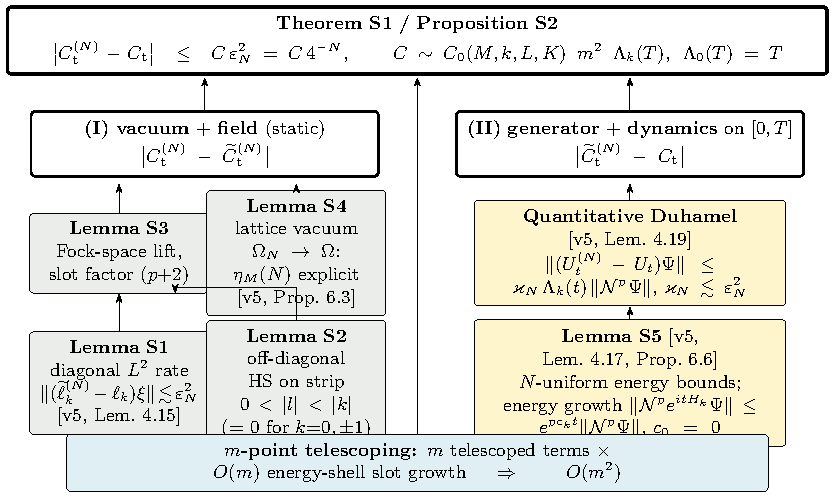
\includegraphics[width=0.95\textwidth]{figure9.pdf}
\caption{\rev{The error budget of Theorem~S1: the master decomposition (Proposition~S1) splits
the correlator error into the static term (I) and the dynamical term (II); the static inputs
are Lemmas~S1--S4, the dynamics module is Lemma~S5 together with the quantitative Duhamel
bound, and the $m$-point telescoping supplies the $O(m^{2})$ factor. Along the momentum-cutoff
route every leaf carries the one-particle rate $\vep_{N}^{2}\propto4^{-N}$; the horizon $T$ enters
only through the energy-growth factor $\Lambda_{k}(T)$ of [v5, Lemma~4.19], linear in $T$ for
$k=0$ and of order $e^{c_{k}T}$ otherwise.}}
\label{fig:errorbudget}
\end{center}
\end{figure}

\noindent\textbf{Theorem~S1 (quantitative discretization bound; target).}~\emph{%
With the data above, along the momentum-cutoff renormalization group and for $2$-regular
smearing ($K\ge5$):}
\begin{enumerate}
\item[(i)] \emph{(chiral Hamiltonian evolution, $k=0$; established, [v5, Proposition~6.3])
For $A,B$ monomials of degrees $d_{A},d_{B}$ in the lattice fermions at scale $M$ and the
dynamics generated by $L_{0}$,}
\begin{equation}\label{eq:target}
  \bigl|C^{(N)}_{t}-C_{t}\bigr|
  \;\le\;(d_{A}+d_{B})\,\eta_{M}(N)\;+\;\tfrac16\,d_{B}\,\Theta_{M}\,|t|\,\vep_{N}^{2},
  \qquad
  \eta_{M}(N)\le\begin{cases}\tfrac{\pi}{4}\,2^{-(N-M)} & \text{on the full algebra},\\[2pt]
  \tfrac{\pi^{2}}{16}\,2^{-2(N-M)} & \text{on the chiral algebra},\end{cases}
\end{equation}
\emph{with $\Theta_{M}=\bigl(\sum_{l\in\Gamma_{M}}\theta(\pm l)|l|^{6}\bigr)^{1/2}$ explicit;
in particular the bound is uniform on $[0,T]$ with a prefactor linear in $T$, and for chiral
observables both terms are of order $4^{-(N-M)}$.}
\item[(ii)] \emph{(local conformal transformations, $k\neq0$; assembled below) There are a
constant $C=C(T,M,k,m,L,K)<\infty$ and $N_{0}\in\N$ such that for all $N\ge N_{0}$ and all
$0\le t_{1},\dots,t_{m}\le T$,}
\begin{equation}\label{eq:targetk}
  \bigl|\,C^{(N)}_{t_{1},\dots,t_{m}}-C_{t_{1},\dots,t_{m}}\,\bigr|
  \;\le\;C(T,M,k,m,L,K)\;\vep_{N}^{2},
  \qquad C(T,M,k,m,L,K)\sim C_{0}(M,k,L,K)\,m^{2}\,\Lambda_{k}(T),
  \quad \Lambda_{k}(T)=\tfrac{e^{c_{k}T}-1}{c_{k}},
\end{equation}
\emph{where $c_{k}$ is the energy-growth constant of [v5, Lemma~4.19] ($c_{0}=0$, so that
$\Lambda_{0}(T)=T$) and $C_{0}$ collects the one-particle constants of [v5, Lemma~4.15] and
the Fock-space slot factors; the rate and the $T$- and $m$-dependence are what the assembly
establishes, the numerical value of $C_{0}$ is not computed here.}
\end{enumerate}
\emph{Consequently, to reach accuracy $\delta$ it suffices that
$C\,\vep_{N}^{2}\le\delta$, i.e., absorbing the fixed factor $L^{2}$ into $C$, that $C\,4^{-N}\le\delta$, i.e.}
\begin{equation}\label{eq:nofdelta}
  N(\delta,T)\;\ge\;\tfrac{1}{2}\log_{2}\!\frac{C}{\delta},
  \qquad
  n(\delta,T)\;=\;2^{N+1}\;\lesssim\;2\,C^{1/2}\,\delta^{-1/2}\;=\;C_{T}\,\delta^{-1/2},
\end{equation}
\emph{which is the convergence $\sim 1/n^{2}$ and the site count $n(\delta,T)\sim
C_{T}\,\delta^{-1/2}$ quoted in the Letter. Along the wavelet renormalization group the
one-particle generator error is of order $\vep_{N}$ for $k\neq0$ [v5, Remark~4.8,
Remark~4.32], so that without re-centring \eqref{eq:nofdelta} degrades to
$n(\delta,T)\sim C_{T}\,\delta^{-1}$ [v5, Remark~6.4(4)]; the re-centred comparison of
[v5, Remark~3.5] restores the exponent $\tfrac12$, and for the Hamiltonian $k=0$ the wavelet
route gives $\vep_{N}^{2}$ once $s$ is $3$-regular ($K\ge9$; attained numerically from
D$10$ on, [v5, Remark~4.32]).} The one-particle bounds evaluated for D$8$ and D$10$ in
Fig.~\ref{fig:waveleterrork} ($k=0$, wavelet route) realize the $4^{-N}$ decay over the
computed range, and Figs.~\ref{fig:momrgerrorM}--\ref{fig:momrgerrorHS} (momentum-cutoff route,
$k=0,1,2$ and the Hilbert--Schmidt part for $k=2,3,4$) show the same decay for $k\neq0$; the
near-term D$10$ figure of the Letter is a one-particle, wavelet-route, $k=0$ statement read
off Fig.~\ref{fig:waveleterrorM}, and Fig.~\ref{fig:corrconv} checks the propagated rate at
the correlator level along the momentum-cutoff route.

\subsection{Static estimates: one-particle, Hilbert--Schmidt, and Fock lifts}\label{sec:static}

We first collect the four \emph{time-independent} estimates of the chain. They quantify, at
a \emph{fixed} scale, the three layers of the construction of~\cite{osborneConformal2021}:
the one-particle generator (Lemma~S1), its off-diagonal Hilbert--Schmidt part (Lemma~S2),
the lift to Fock space (Lemma~S3), and the lattice vacuum (Lemma~S4). For each we state the
bound and its source. We write
$\widetilde\ell^{(N)}_{\pm,k}=R^N_\infty\,\ell^{(N)}_{\pm,k}(R^N_\infty)^{*}$ for the
scale-matched one-particle KS operators and $L^{(N)}_{k}=\ud\Gamma(\ell^{(N)}_k)$ for their
second quantization.

\medskip\noindent\textbf{Lemma~S1 (one-particle generator rate; [v5, Lemma~4.15, Thm~4.16]).}~\emph{%
Along the momentum-cutoff renormalization group, for every $\delta_{\!s}>0$ and every
one-particle vector $\xi$ in the Sobolev space $h^{1+\delta_{\!s}}$,}
\begin{equation}\label{eq:wp1}
  \bigl\lVert(\widetilde\ell^{(N)}_{\pm,k}-\ell_{\pm,k})\,\xi\bigr\rVert
  \;\le\; C_1(k,L)\,\vep_{N}^{\min\{\delta_{\!s},2\}}\,\lVert\xi\rVert_{h^{1+\delta_{\!s}}},
\end{equation}
\emph{and the rate is sharp. For $\xi$ of spectral support up to the observation scale $M$,
$\lVert\xi\rVert_{h^{1+\delta_{\!s}}}\le(1+\mathrm{const}\,2^{M})^{1+\delta_{\!s}}\lVert\xi\rVert$,
and no scaling function enters; regularity of $s$ is needed only through the smearing of
the observables, where $2$-regularity ($K\ge5$) gives $\delta_{\!s}=2$ [v5, Remark~6.4(3)].}

\noindent\emph{Source and mechanism.} The matrix elements of $\widetilde\ell^{(N)}_{\pm,k}$
in the plane-wave basis are explicit, and the difference to $\ell_{\pm,k}$ is the finite sum
\cite[eq.~(212)]{osborneConformal2021} of the deviations
$\vep_{N}^{-1}\sin(\vep_{N}(l\mp\tfrac k2))-(l\mp\tfrac k2)=O(\vep_{N}^{2}|l\mp\tfrac k2|^{3})$,
which is where the rate $\vep_{N}^{2}$ and the weight $h^{1+\delta_{\!s}}$ come from
[v5, Lemma~4.15]. This is the $L^{2}$-error plotted in
Figs.~\ref{fig:momrgerrorM} and~\ref{fig:momrgerrork} ($c=\tfrac12,1$, momentum-cutoff route).
Along the wavelet renormalization group the analogous statement is [v5, Lemma~4.7, Theorem~4.9]
with the rate $\vep_{N}^{2}$ for $k=0$ (Figs.~\ref{fig:waveleterrorM}, \ref{fig:waveleterrork},
$c=0$) but only $\vep_{N}$ for $k\neq0$ [v5, Remark~4.8, Remark~4.32]; the published domination
argument \cite[Lemma~4.5, eqs.~(204)--(210)]{osborneConformal2021} is replaced in [v5,
Lemma~3.14, Corollary~3.15] by an $N$-uniform majorant.\hfill$\square$

\medskip\noindent\textbf{Lemma~S2 (off-diagonal Hilbert--Schmidt part).}~\emph{%
Along the momentum-cutoff renormalization group the off-diagonal (pair-creation) block of the
one-particle generator difference satisfies}
\begin{equation}\label{eq:wp2}
  \bigl\lVert(\widetilde\ell^{(N)}_{\pm,k}-\ell_{\pm,k})_{\pm\mp}\bigr\rVert_2^2
  \;\le\; C_2(k)\,\vep_{N}^{4},
\end{equation}
\emph{a sum over the finite off-diagonal strip $0<|l|<|k|$ \cite[eq.~(212)]{osborneConformal2021},
[v5, Lemma~4.15]; in the Neveu--Schwarz sector it vanishes identically for the M\"obius
generators $k=0,\pm1$ (i.e.\ $L_{-1},L_0,L_1$), which therefore incur no off-diagonal cost
[v5, Remark~4.22].}

\noindent\emph{Source and mechanism.} The Hilbert--Schmidt norm is restricted by the step
functions $\theta(\pm(l\mp k))\theta(\mp l)$ to the integer strip $0<|l|<|k|$, which has
$2(|k|-1)$ points and is empty for $k=0,\pm1$; each summand is $O(\vep_{N}^{2})$ by the same
$\sin(x)/x$ expansion as in Lemma~S1, and the index set being finite, no tail summation is
needed. This is the HS-error of Fig.~\ref{fig:momrgerrorHS}, which indeed vanishes for
$k=0,\pm1$. We note that the stronger published statement \cite[Rmk~4.14]{osborneConformal2021},
that for the M\"obius generators the wavelet renormalization group alone suffices, does not
follow from its proof (the Hardy projections do not preserve the wavelet space); only the
vanishing of the Hilbert--Schmidt part is used here [v5, Remark~4.22].\hfill$\square$

\medskip\noindent\textbf{Lemma~S3 (second-quantization lift; \cite[eq.~(200)]{osborneConformal2021}).}~\emph{%
Let $o=\ell_{\pm,k}$ and $\widetilde o^{(N)}=\widetilde\ell^{(N)}_{\pm,k}$, and let
$\eta_1,\dots,\eta_p$ be one-particle vectors localized at scale $M$; write
$\lVert\eta\rVert_{M}$ for the associated one-particle Sobolev norm of Lemma~S1. Then}
\begin{equation}\label{eq:wp3}
\begin{split}
  \bigl\lVert\ud\Gamma(\widetilde o^{(N)}-o)\,a^\dagger(\eta_1)\cdots a^\dagger(\eta_p)\Omega_0\bigr\rVert
  &\;\le\;\Bigl(\textstyle\sum_{q=1}^p \lVert(\widetilde o^{(N)}-o)_{\mathrm{diag}}\eta_q\rVert
  \;+\;(p+2)\,\lVert(\widetilde o^{(N)}-o)_{+-}\rVert_2 \\
  &\;+\;p\,\lVert(\widetilde o^{(N)}-o)_{-+}\rVert_2\Bigr)\!\!\prod_{q=1}^p\lVert\eta_q\rVert_M ,
\end{split}
\end{equation}
\emph{so by Lemmas~S1--S2 the right-hand side is $\le C_3(k,L)\,(p+2)\,\vep_{N}^{2}
\prod_q\lVert\eta_q\rVert_M$.}

\noindent\emph{Source and mechanism.} Because $L^{(N)}_k=\ud\Gamma(\ell^{(N)}_k)$ is
\emph{bilinear} in the fermions, its action on a $p$-particle vector is a sum over the $p$
slots plus the two off-diagonal (pair-creation/annihilation) slots; the diagonal blocks enter
through their norm on the one-particle vectors (Lemma~S1) and the off-diagonal blocks through
their Hilbert--Schmidt norm (Lemma~S2), with the explicit slot prefactor $(p+2)$ on the
pair-creation term. This inequality is unaffected by the revision of the one-particle
estimates. The per-generator factor of the particle number is what propagates into the
dynamics (each $B_t$ acts on a fixed energy shell) and, in the $m$-point case, into the
$O(m^2)$ growth of the assembled constant.\hfill$\square$

\medskip\noindent\textbf{Lemma~S4 (lattice-vacuum rate; [v5, Proposition~6.3, Corollary~3.19]).}~\emph{%
For $O\in\fA_{M}$ a monomial of degree $d$ in the lattice fermions and the scale-matching
maps $\alpha^M_N$, the lattice vacua $\omega^{(N)}_{0,\pm}$ approach the scaling-limit state
$\omega_\pm$ at the rate}
\begin{equation}\label{eq:wp4}
  \bigl|\,\omega^{(N)}_{0,\pm}(\alpha^M_N(O))-\omega_\pm(\alpha^M_\infty(O))\,\bigr|
  \;\le\; d\;\eta_{M}(N),
  \qquad
  \eta_{M}(N)=\max_{l\in\Gamma_{M}}\bigl\lVert S^{(N)}_{0}(l)-S(l)\bigr\rVert,
\end{equation}
\emph{with $\eta_{M}(N)\le\tfrac{\pi}{4}2^{-(N-M)}$ on the full two-component algebra and
$\eta_{M}(N)\le\tfrac{\pi^{2}}{16}2^{-2(N-M)}$ on the chiral algebra.}

\noindent\emph{Source and mechanism.} Both states are quasi-free, so the left-hand side is a
polynomial in matrix elements of the one-particle symbols $S^{(N)}_{0},S$, and the symbols are
explicit along the momentum-cutoff route: the deviation is a sine of the ratio
$\vep_{N}/\vep_{M}=2^{-(N-M)}$, of first order on the full algebra and of second order on the
chiral algebra, because the chiral entanglement of the finite-scale vacuum is the obstruction
[v5, Proposition~6.3, Remark~6.4(2)]. Both error sources of the master decomposition therefore
scale in the renormalization depth $r=N-M$ rather than in $N$ alone
[v5, Remark~6.4(1)].\hfill$\square$

\medskip\noindent
Together, Lemmas~S1--S4 control every \emph{static} ingredient of the master decomposition
at rate $\vep_{N}^{2}$ (on chiral observables, and up to the first-order vacuum term on the
full algebra): the field discretization $\widetilde A-A$ and the vacuum $\Omega_N\to\Omega$
(Lemmas~S3--S4), and the instantaneous generator difference $H^{(N)}_k-H_k$ acting on a fixed
energy shell (Lemmas~S1--S3). What remains is to propagate the generator difference through
the \emph{unbounded} Heisenberg dynamics over $[0,T]$, uniformly in $t$ and for all $k$.

\subsection{The Heisenberg dynamics over \texorpdfstring{$[0,T]$}{[0,T]}}\label{sec:wp5}

The static estimates above control the discretization of the generators, fields, and vacuum
\emph{at a fixed time}. What the correlator requires in addition is that this control survive
\emph{conjugation by the unitary Heisenberg flow}
$\widetilde B_t=e^{itH_k^{(N)}}\,\widetilde B\,e^{-itH_k^{(N)}}$ versus
$B_t=e^{itH_k}\,B\,e^{-itH_k}$, generated by the \emph{unbounded} self-adjoint
$H_k=L_k+L_{-k}$, uniformly on a horizon $[0,T]$. For the Hamiltonian $k=0$ this is done with
all constants in [v5, Proposition~6.3]; for $k\neq0$ the three ingredients are established
in [v5] --- essential self-adjointness (Corollary~4.18), $N$-uniform energy bounds (Lemma~4.17,
Proposition~6.6) and the energy-growth/Duhamel estimate (Lemma~4.19) --- and are combined
here. Throughout, $\Psi$ ranges over the finite-particle core
$\fA^{\mathrm{alg}}\subset\cF_{\ua}(\cH)$ and $\mathcal{N}:=\1+L_{0}$, $\mathcal{N}^{(N)}:=\1+L_{0}^{(N)}$.

\medskip\noindent\textbf{Well-posedness of the flows.}~For each order $k$ and each $N$
(including $N=\infty$), the self-adjoint combinations of Koo--Saleur generators
$H_k^{(N)}=L_k^{(N)}+L_{-k}^{(N)}$ and $i(L_k^{(N)}-L_{-k}^{(N)})$ are essentially
self-adjoint on every core for $\mathcal{N}^{(N)}$, in particular on $\fA^{\mathrm{alg}}$, and the
unitary groups $U_t^{(N)}=e^{itH_k^{(N)}}$, $U_t=e^{itH_k}$ are well defined. This is
Nelson's commutator theorem applied with $\mathcal{N}$ [v5, Corollary~4.18]: its first hypothesis
is the linear energy bound of Lemma~S5 below and its second the form bound on the commutator
$[\mathcal{N},H_{k}]$, which is again a Koo--Saleur bilinear. (The earlier route through analytic
vectors of the finite-particle core, \cite[Cor.~4.3]{osborneConformal2021}, does not close as
stated, because the pair-creation terms raise the particle number; see the discussion in
[v5] preceding Corollary~4.18.) The non-self-adjoint $L_k$ alone ($k\neq0$) generates no
unitary group; only the self-adjoint combination $H_k=L_k+L_{-k}$ is simulated, exactly as in
the Letter.

\medskip\noindent\textbf{Lemma~S5 (uniform linear energy bounds and energy growth;
[v5, Lemma~4.17, Proposition~6.6, Lemma~4.19]).}~\emph{Let $s$ be $1$-regular ($K\ge3$).
There are constants $b_k,c_k<\infty$, independent of $N\in\N\cup\{\infty\}$, with}
\begin{align}
  \lVert L_k^{(N)}\Psi\rVert &\;\le\; b_k\,\lVert\mathcal{N}^{(N)}\Psi\rVert,
  \label{eq:linbound}\\[2pt]
  \pm\,H_k^{(N)}\;=\;\pm\bigl(L_k^{(N)}+L_{-k}^{(N)}\bigr) &\;\le\; b_k\,\mathcal{N}^{(N)}
  \quad\text{(as quadratic forms),}
  \label{eq:qformbound}
\end{align}
\emph{for the single generators and, with a constant $C_{X}$ depending on the smearing
function $X$, for the smeared KS approximants. Consequently the flow propagates the energy at
most exponentially: for $p\in\N$,}
\begin{equation}\label{eq:gronwall}
  \bigl\lVert(\mathcal{N}^{(N)})^{p}\,e^{itH_k^{(N)}}\Psi\bigr\rVert
  \;\le\; e^{p\,c_k|t|}\,\bigl\lVert(\mathcal{N}^{(N)})^{p}\Psi\bigr\rVert,
  \qquad c_{0}=0 .
\end{equation}

\noindent\emph{Source.} The bounds~\eqref{eq:linbound}--\eqref{eq:qformbound} are the
lattice counterparts of the Virasoro \emph{linear energy bounds} of Buchholz and
Schulz-Mirbach~\cite{buchholzSchulzMirbach1990} in the form used by
Carpi~\cite{carpiVirasoroNets2004}; that they hold for the KS approximants \emph{uniformly in
the scale} is [v5, Lemma~4.17] for a single order $k$ and [v5, Proposition~6.6] for smeared
generators, under $1$-regularity of $s$. This closes the gap in the published proof of
\cite[Thm~6.3]{osborneConformal2021}, where such a bound had been asserted. The mechanism is
elementary: the one-particle KS symbol is $\vep_{N}^{-1}\sin(\vep_{N}(l\mp\tfrac k2))$ and the
one-particle energy $\vep_{N}^{-1}|\sin(\vep_{N}l)|$-like, so $|\sin(a+b)|\le|\sin a|+|\sin b|$
and $|\sin x|\le|x|$ give a relative bound with constants that do not depend on the spacing;
second quantization transports it to $\ud\Gamma_{S}$ with the same constants because the
number operator is dominated by $L_{0}^{(N)}$ uniformly in $N$. The energy
growth~\eqref{eq:gronwall} is [v5, Lemma~4.19(i)], a Gr\"onwall argument on
$\lVert(\mathcal{N}^{(N)})^{p}\Psi_{t}\rVert^{2}$ using the form bound on $i[L_{0}^{(N)},H_{k}^{(N)}]$,
with $c_{0}=0$ because $[L_{0},H_{0}]=0$. Thus a state of bounded energy stays, for all
$t\le T$, inside a horizon-dependent but $N$-independent energy shell, on which the static
rates of Lemmas~S1--S3 apply uniformly. \hfill$\square$

\medskip\noindent\textbf{Quantitative Duhamel (the rate-carrier; [v5, Lemma~4.19(ii)]).}~%
Let $\Psi\in\fA^{\mathrm{alg}}$ and let $\varkappa_{N}$ be a bound
$\lVert(H_k^{(N)}-H_k)\Phi\rVert\le\varkappa_{N}\lVert\mathcal{N}^{p}\Phi\rVert$ for the generator
difference relative to the $p$-th power of the energy. Then, for all $t$,
\begin{equation}\label{eq:quantduhamel}
  \bigl\lVert(U_t^{(N)}-U_t)\Psi\bigr\rVert
  \;\le\;\varkappa_{N}\,\Lambda_{k,p}(t)\,\lVert\mathcal{N}^{p}\Psi\rVert,
  \qquad \Lambda_{k,p}(t)=\frac{e^{p\,c_k|t|}-1}{p\,c_k}\ \ (=|t|\ \text{for}\ k=0).
\end{equation}
On the common core the Duhamel identity
$(U_t^{(N)}-U_t)\Psi=i\int_0^t U_{t-s}^{(N)}\,(H_k^{(N)}-H_k)\,U_s\Psi\,\ud s$ holds, the
integrand being well defined because $U_s\Psi$ stays in the domain of $\mathcal{N}^{p}$
(well-posedness above) and $U_{t-s}^{(N)}$ is \emph{unitary}; inserting the relative bound
and the energy growth~\eqref{eq:gronwall} and integrating gives~\eqref{eq:quantduhamel}. The
input $\varkappa_{N}$ is supplied by Lemmas~S1--S3 with $p=1+\delta_{\!s}$ relative powers of the
energy: $\varkappa_{N}\le C_{1}(k,L)\,\vep_{N}^{2}$ for $2$-regular smearing. Two special cases
are worth isolating. First, for the M\"obius generators $k=0,\pm1$ the off-diagonal
Hilbert--Schmidt contribution of Lemma~S2 vanishes (Fig.~\ref{fig:momrgerrorHS}), so the
generator difference is purely diagonal. Second --- a \emph{distinct} property --- for the
strict Hamiltonian case $k=0$ one has $[L_0,H_0]=0$, hence $c_0=0$ and the energy shell is
\emph{dynamically invariant}: the prefactor reduces to the linear-in-$T$ behavior
$\Lambda_{0,p}(T)=T$, which is the $k=0$ bound of \cite[Rmk~4.21]{osborneConformal2021} and
the dynamics term of [v5, Proposition~6.3]. These are not the same statement: off-diagonal
Hilbert--Schmidt vanishing holds for all of $k=0,\pm1$, but dynamical shell-invariance and the
linear-in-$T$ prefactor hold for $k=0$ \emph{only} --- for $k=\pm1$ one has
$[L_0,L_{\pm1}]=\mp L_{\pm1}\neq0$, so $c_{\pm1}\neq0$ and the energy genuinely grows as
$e^{c_{\pm1}T}$; the one-particle constant is $c_{\sigma,k}\le C_{L}\,\sigma|k|\langle k\rangle^{\sigma+2}$
[v5, Lemma~4.12].

\medskip\noindent\textbf{Conjugation of the observable.}~For $\widetilde B$ a smeared
(bounded) field at observation scale $M$,
\begin{equation}\label{eq:conjbound}
  \bigl\lVert(\widetilde B_t-B_t)\,\Psi\bigr\rVert
  \;\le\; C'(M,k)\,\Lambda_{k,p}(T)\,\lVert\widetilde B\rVert_{\!*}\,\vep_{N}^{2},
  \qquad 0\le t\le T,
\end{equation}
where $\lVert\,\cdot\,\rVert_{\!*}$ is the appropriate one-particle/Fock weight of the
field and $\Psi$ runs over the finite-energy core. To see this, apply the three-term split
of the conjugation that appears in~\eqref{eq:conjsplit},
\[
  \widetilde B_t-B_t
  \;=\;(U_t^{(N)}-U_t)\,\widetilde B\,U_t^{(N)*}
  \;+\;U_t\,(\widetilde B-B)\,U_t^{(N)*}
  \;+\;U_t\,B\,(U_t^{(N)*}-U_t^{*}),
\]
and evaluate on the finite-particle vacuum (or finite-energy $\Psi$). The bounded smeared
$\widetilde B$ acting on such a vector shifts the particle number by a \emph{bounded}
amount and thus produces a vector of \emph{finite energy}, so all three terms are finite.
The outer two are bounded by~\eqref{eq:quantduhamel} (using $\lVert\mathcal{N}^{p}\widetilde B\,\Psi\rVert$
and $\lVert\mathcal{N}^{p}B\,\Psi\rVert$ as the relevant weights), and the middle term by the static
field estimate $\lVert(\widetilde B-B)\Psi\rVert\le C\,\vep_{N}^{2}$ of Lemmas~S1/S3 with
$U_t,U_t^{(N)*}$ unitary. Collecting the three constants gives~\eqref{eq:conjbound}.

\medskip\noindent\textbf{Trotter--Kato as a qualitative cross-check.}~%
The strong-resolvent convergence $H_k^{(N)}\to H_k$ established in
\cite{osborneConformal2021} and [v5, Theorem~4.16, Corollary~4.18], combined with the uniform
energy bounds~\eqref{eq:linbound}--\eqref{eq:qformbound}, already implies $U_t^{(N)}\to U_t$
strongly and uniformly for $t$ in compact intervals, by the Trotter--Kato theorem. This
serves only as an independent consistency check: it reproduces the \emph{qualitative}
statement but \emph{carries no rate}, and is therefore strictly weaker than the quantitative
Duhamel bound~\eqref{eq:quantduhamel}, which is what feeds the accuracy estimate. In
particular, no rate is at any point extracted from strong-resolvent convergence.

\medskip\noindent\textbf{Net effect.}~The steps above replace the $k=0$-only, one-particle
Duhamel estimate of \cite[Rmk~4.21]{osborneConformal2021} by an \emph{all-$k$}, full-Fock
conjugation bound~\eqref{eq:conjbound} that is uniform on $[0,T]$ with the horizon dependence
$\Lambda_{k,p}(T)$ of [v5, Lemma~4.19] (linear in $T$ in the strict Hamiltonian case $k=0$,
where the energy shell is dynamically invariant). This is the dynamical input to the
assembly: the energy weight of the dynamically evolved state is the $T$-factor that,
multiplied by the static $\vep_{N}^{2}$ rate of Lemmas~S1--S4 and the $O(m^2)$ telescoping
below, produces the final bound.

\subsection{Multi-point telescoping and the master decomposition}\label{sec:assembly}

The single-correlator bounds of the preceding subsections (the one-particle rate of
Lemmas~S1--S2, the second-quantization lift of Lemma~S3, the vacuum rate of Lemma~S4, and
the uniform-in-$t$ dynamics of Lemma~S5 and~\eqref{eq:conjbound}) are now assembled. We
first treat a general $m$-point configuration, then collect everything into the master error
estimate.

\medskip\noindent\textbf{$m$-point telescoping.}~Let $\widetilde A_1,\dots,\widetilde A_m$
be discretized smeared observables localized at scale $M$ (bounded lattice fields), with
continuum counterparts $A_1,\dots,A_m\in\fA_M$, evolved to times $0\le t_1,\dots,t_m\le T$
under $\widetilde A_{p,t_p}=U^{(N)}_{t_p}\widetilde A_p\,U^{(N)*}_{t_p}$ and
$A_{p,t_p}=U_{t_p}A_p\,U^*_{t_p}$, with $U_t=e^{itH_k}$, $U^{(N)}_t=e^{itH^{(N)}_k}$ as
above. The object of interest is the lattice correlator
\begin{equation}\label{eq:mpoint}
  C^{(N)}_{\mathbf t}\;=\;\bigl\langle\Omega_N\,\big|\,\widetilde A_{1,t_1}\cdots\widetilde A_{m,t_m}\,\big|\,\Omega_N\bigr\rangle,
  \qquad
  C_{\mathbf t}\;=\;\bigl\langle\Omega\,\big|\,A_{1,t_1}\cdots A_{m,t_m}\,\big|\,\Omega\bigr\rangle .
\end{equation}
Following the telescoping of~\cite[Thm~6.3, eqs.~(236)--(237)]{osborneConformal2021}
(now unconditional, [v5, Theorem~6.5]), we split the product factor by factor,
\begin{equation}\label{eq:telescope}
  \widetilde A_{1,t_1}\cdots\widetilde A_{m,t_m}-A_{1,t_1}\cdots A_{m,t_m}
  \;=\;\sum_{p=1}^{m}
  A_{1,t_1}\cdots A_{p-1,t_{p-1}}\,
  \bigl(\widetilde A_{p,t_p}-A_{p,t_p}\bigr)\,
  \widetilde A_{p+1,t_{p+1}}\cdots\widetilde A_{m,t_m},
\end{equation}
together with the analogous replacement $\Omega_N\to\Omega$ of the vacuum (Lemma~S4). The
continuum prefactors and lattice postfactors in~\eqref{eq:telescope} act on a \emph{fixed}
finite-energy shell (the smeared $A_p$ raise the particle number by a bounded amount and
shift $L_0$ by a bounded amount), so by the uniform energy bounds of Lemma~S5 the operator
products are bounded uniformly in $N$. Hence
\begin{equation}\label{eq:mpointbound}
  \bigl|C^{(N)}_{\mathbf t}-C_{\mathbf t}\bigr|
  \;\le\;
  \sum_{p=1}^{m}\,\bigl\lVert(\widetilde A_{p,t_p}-A_{p,t_p})\,\Psi_p\bigr\rVert
  \;+\;\bigl|\,\omega^{(N)}-\omega\,\bigr|(\,\cdots\,)
  \;\le\; C(T,M,k)\,m^2\,\vep_{N}^{2},
\end{equation}
where $\Psi_p$ is the (energy-bounded) vector produced by the factors to the right of slot
$p$. The two powers of $m$ arise as follows: there are $m$ telescoped
terms~\eqref{eq:telescope}, and each per-factor error
$\lVert(\widetilde A_{p,t_p}-A_{p,t_p})\Psi_p\rVert$ already carries one factor of $m$
through the Lemma~S3 slot count, since $\Psi_p$ lives on an energy shell whose particle
number grows linearly with the number $m{-}p$ of fields to its right. Thus the per-factor
errors are $O(m)$ and there are $O(m)$ of them, giving the overall $O(m^2)$ that the
Letter quotes. For the chiral Hamiltonian evolution the vacuum term is instead the explicit
$(d_{A}+d_{B})\eta_{M}(N)$ of [v5, Proposition~6.3], linear in the degrees.

\medskip\noindent\textbf{Proposition~S2 (assembly of the target rate).}~\emph{Under the
hypotheses of Theorem~S1(ii) --- a free-fermion CFT ($c=\tfrac12$; or $c=0,1$), the
momentum-cutoff renormalization group with $2$-regular smearing ($K\ge5$), a generator order
$k$, a localization scale $M$, an $m$-point configuration of smeared fields in $\fA_M$, and
a horizon $T$ --- the static estimates (Lemmas~S1--S4), the dynamics module (Lemma~S5
and~\eqref{eq:quantduhamel}), and the $m$-point telescoping~\eqref{eq:mpointbound} combine
to give the target bound~\eqref{eq:targetk}: there exist $C=C(T,M,k,m,L,K)<\infty$ and $N_0$
such that for all $N\ge N_0$ and $0\le t_1,\dots,t_m\le T$,}
\begin{equation}\label{eq:masterrate}
  \bigl|C^{(N)}_{\mathbf t}-C_{\mathbf t}\bigr|\;\le\;C\,\vep_{N}^{2},
\end{equation}
\emph{with the constant $C$ left in the factored form below. For $k=0$ and two-point
functions of monomials the statement is Theorem~S1(i), with every constant explicit.}

\medskip\noindent\emph{Sketch.}~Insert between $C^{(N)}_{\mathbf t}$ and $C_{\mathbf t}$ the
intermediate object $\widetilde C^{(N)}_{\mathbf t}$ that uses the \emph{continuum} vacuum
and continuum fields but the lattice-pushed (approximating Bogoliubov) dynamics, exactly as
in Proposition~S1, and telescope,
\[
  \bigl|C^{(N)}_{\mathbf t}-C_{\mathbf t}\bigr|
  \;\le\;
  \underbrace{\bigl|C^{(N)}_{\mathbf t}-\widetilde C^{(N)}_{\mathbf t}\bigr|}_{\text{vacuum (Lem.~S4) + field discretization (Lems.~S1--S3)}}
  \;+\;
  \underbrace{\bigl|\widetilde C^{(N)}_{\mathbf t}-C_{\mathbf t}\bigr|}_{\text{generator/dynamics over }[0,T]\ \text{(Lem.~S5)}}.
\]
Each atomic error is $\le(\text{const})\,\vep_{N}^{2}$: the field/vacuum terms by
Lemmas~S1--S4 (the one-particle rate of Lemma~S1 with the off-diagonal Hilbert--Schmidt rate
of Lemma~S2, lifted to Fock space by the bound of Lemma~S3, plus the explicit vacuum rate of
Lemma~S4), and the dynamics term by the quantitative Duhamel estimate~\eqref{eq:quantduhamel},
which confines the evolution to an energy shell via the uniform energy bounds of Lemma~S5,
yielding the horizon factor $\Lambda_{k,p}(T)$. The factors multiply: $C$ is the product of
the one-particle constant $C_{1}(k,L)$ of Lemma~S1, the horizon factor of Lemma~S5, the
combinatorial factor $m^2$ of~\eqref{eq:mpointbound}, and the Sobolev weight of the vectors
$\widetilde A_p\Omega$. Summing the telescoped
contributions~\eqref{eq:telescope}--\eqref{eq:mpointbound} gives~\eqref{eq:masterrate}, which
is the bound asserted in Theorem~S1(ii). What is \emph{established} is the rate $\vep_{N}^{2}$
(equivalently the exponent $\tfrac12$ in $n(\delta,T)$) together with the explicit $T$- and
$m$-dependence; the numerical value of the prefactor for $k\neq0$ is not computed
here.\hfill$\square$

\subsection{Reconciliation with the Letter and inversion of the rate}\label{sec:reconcile}

Inverting~\eqref{eq:masterrate} gives the quantitative content used in the Letter. To reach
accuracy $\delta$ it suffices that $C\,\vep_{N}^{2}\le\delta$, i.e., absorbing the fixed factor $L^{2}$ into $C$, that $C\,4^{-N}\le\delta$, i.e.
\begin{equation}\label{eq:invert}
  N(\delta,T)\;\ge\;\tfrac12\,\log_2\!\frac{C}{\delta},
  \qquad\Longrightarrow\qquad
  n(\delta,T)\;=\;2^{N+1}\;\lesssim\;2\,C^{1/2}\,\delta^{-1/2}
  \;=\;C_T\,\delta^{-1/2},
\end{equation}
recovering~\eqref{eq:nofdelta}. Here $\delta$ denotes the target \emph{accuracy}; regularity
enters only through the hypothesis on the smearing ($K\ge5$). Thus
\begin{equation}\label{eq:rateletter}
  n(\delta,T)\;\sim\;C_T\,\delta^{-1/2},
\end{equation}
the resource scaling quoted in the Letter and consistent with the
$\mathrm{error}\sim\vep_{N}^{2}\sim 1/n^{2}$ convergence. The external parameters enter the
prefactor $C_T=2\,C^{1/2}$ transparently. For the chiral Hamiltonian evolution ($k=0$)
everything is explicit [v5, Remark~6.4]: with $d=d_{A}+d_{B}$ the depth must satisfy
$N-M\ge\tfrac12\log_{2}\bigl(C\,d\,(1+T)/\delta\bigr)$, so that
$n(\delta,T)\sim 2^{M+1}\sqrt{C\,d\,(1+T)/\delta}$ and the horizon enters as $\sqrt{1+T}$; the
prefactor $2^{M}$ is fixed by $M<N$ and by the localization of the smearing function,
$\vep_{M}(2K-1)\lesssim L$. For the local conformal transformations ($k\neq0$) the horizon
enters through $\Lambda_{k,p}(T)^{1/2}$, i.e.\ as $e^{c_{k}T/2}$, the point count $m$ as
$m$, and the generator order $k$, localization scale $M$, lattice length $L$ and Daubechies
order $K$ through the one-particle constant $C_{1}(k,L)$ of Lemma~S1 and the Sobolev weights;
the numerical value of that prefactor is not computed here. Along the wavelet renormalization
group the generator error for $k\neq0$ is of order $\vep_{N}$ rather than $\vep_{N}^{2}$
unless the comparison is re-centred, so that~\eqref{eq:rateletter} degrades to
$n(\delta,T)\sim C_{T}\,\delta^{-1}$ [v5, Remark~6.4(4)]: localization in real space, which is
what the wavelet route buys, is paid for in qubits unless one re-centres [v5, Remark~3.5].
The near-term estimate of the Letter (a D$10$ wavelet reaching $\delta=\tfrac12$ on $128$
sites at observation scale $M=3$) is read off the one-particle wavelet-route data for $k=0$
in Fig.~\ref{fig:waveleterrorM}, for which the rate $\vep_{N}^{2}$ is available ($K=10\ge9$);
we note that the localization constraint $2^{M}\gtrsim2K-1$ of
\cite[Rmk~4.20]{osborneConformal2021} and [v5, Remark~6.4(3)] is not met at $M=3$ for $K=10$,
so that the observables of that estimate are wavelet details wrapped around the circle
rather than strictly localized fields; the register size of the estimate is unaffected.

\subsection{Relation to the numerical figures}\label{sec:numerics}

The one-particle rate that drives the whole estimate (Lemmas~S1--S2) is exactly the
quantity measured in Figs.~\ref{fig:waveleterrorM}--\ref{fig:momrgerrorHS}. These figures
are therefore the numerical corroboration of the one-particle ingredient on which
Proposition~S2 rests; Fig.~\ref{fig:corrconv} complements them with a direct
\emph{correlator-level} check of the assembled bound.
\begin{itemize}
\item Figures~\ref{fig:waveleterrorM} and~\ref{fig:waveleterrork} ($c=0$, wavelet RG) plot
the diagonal $L^2$-norm error between $L_0$ and $L^{(N)}_0$ on one-particle wavelet-detail
states up to scale $M$, as a function of $N$; the slope realizes the $4^{-N}$ decay for the
Hamiltonian $k=0$, and Fig.~\ref{fig:waveleterrork} resolves the dependence on the Sobolev
regularity of the Daubechies scaling function, in agreement with the thresholds of
[v5, Remark~3.13]. For $k\neq0$ the wavelet route gives only $2^{-N}$ unless re-centred
[v5, Remark~4.32]; no such data are shown.
\item Figures~\ref{fig:momrgerrorM} and~\ref{fig:momrgerrork} ($c=\tfrac12,1$,
momentum-cutoff RG) plot the diagonal $L^2$-norm error for $L_k$ versus $L^{(N)}_k$ on
momentum states up to scale $M$, against $N$ and against the generator order $k$; these
exhibit the $4^{-N}$ diagonal rate of Lemma~S1 for $k=0,1,2$ in the non-trivial
representations.
\item Figure~\ref{fig:momrgerrorHS} plots the \emph{off-diagonal} Hilbert--Schmidt error of
Lemma~S2, a finite sum over the strip $0<|l|<|k|$. As marked in its caption, this error
\emph{vanishes for the M\"obius generators} $k=0,\pm1$ [v5, Remark~4.22]: the generators
$L_{-1},L_0,L_1$ incur no off-diagonal cost, so for the M\"obius subalgebra the Lemma~S3 lift
reduces to the diagonal term alone.
\end{itemize}
Thus the figures measure the one-particle behavior (diagonal $L^2$ and off-diagonal
Hilbert--Schmidt) that, propagated through Lemmas~S3--S5 and the telescoping, produces the
correlator rate~\eqref{eq:masterrate} and the resource scaling~\eqref{eq:rateletter}.
Figure~\ref{fig:corrconv} verifies the propagated rate directly at the correlator level: the
two-point function of smeared fields evolved by $H_k$ converges at $4^{-N}$ uniformly over
the plotted horizon, and the late-time growth at $k=2$ visualizes the energy-growth
mechanism of Lemma~S5.

\subsection*{Inputs and new estimates}

We list the cited inputs and the estimates assembled here.

\medskip\noindent\textbf{Cited inputs.}~From~\cite{osborneConformal2021} and its revised
version~\cite{osborneConformalRevised2026}: the strong / strong-resolvent convergence of the
KS approximants and of the correlation functions, uniform on compact time intervals
(\cite[Thms~4.6, 4.11, 4.16, 6.1, 6.3]{osborneConformal2021}; [v5, Thms~4.16, 4.25, 6.1, 6.5]);
the sharp one-particle rate $\vep_{N}^{\min\{\delta_{\!s},2\}}$ along the momentum-cutoff route
[v5, Lemma~4.15, Thm~4.16] and the wavelet-route rates [v5, Remark~4.8, Remark~4.32]; the
regularity thresholds [v5, Definition~3.12, Remark~3.13]; the Fock-space lift
\cite[eq.~(200)]{osborneConformal2021}; the explicit lattice-vacuum rate and the explicit
correlator bound for the chiral Hamiltonian evolution [v5, Proposition~6.3] with its qubit
budget [v5, Remark~6.4]; the $N$-uniform linear energy bounds [v5, Lemma~4.17,
Proposition~6.6]; essential self-adjointness by Nelson's commutator theorem
[v5, Corollary~4.18] (Reed--Simon~\cite{reedSimonMethods}, Thm~X.37); the energy-growth and
Duhamel estimates [v5, Lemmas~4.12 and~4.19]; Araki / Shale--Stinespring
\cite{arakiQuasifree1970,shaleStinespring1965} quasi-free implementability (off-diagonal
Hilbert--Schmidt condition); Daubechies~\cite{daubechiesTenLecturesWavelets1992} for the
Sobolev exponents; and the continuum Virasoro linear energy bounds
(Buchholz--Schulz-Mirbach~\cite{buchholzSchulzMirbach1990}; Carpi~\cite{carpiVirasoroNets2004})
of which the lattice bounds are the uniform counterparts.

\medskip\noindent\textbf{Assembled here.}~The propagation of the one-particle rate to the
\emph{full $m$-point correlator} for the local conformal transformations $k\neq0$ with the
explicit decomposition~\eqref{eq:masterrate}: the conjugation bound~\eqref{eq:conjbound}
carried by the self-adjoint generator $H_k=L_k+L_{-k}$ (energy-shell confinement and the
Duhamel estimate of [v5, Lemma~4.19], with Trotter--Kato serving only as a qualitative
cross-check, \emph{not} as the rate-carrier); the $m$-point telescoping yielding $O(m^2)$; and
the assembly into the resource scaling $n(\delta,T)\sim C_T\,\delta^{-1/2}$ along the
momentum-cutoff route, with the wavelet-route caveat stated. For $k=0$ nothing is assembled:
the bound is [v5, Proposition~6.3] with all constants. The strong-resolvent convergence
carries \emph{no} rate; the rate originates entirely from the one-particle estimate, and the
value of the prefactor for $k\neq0$ is not computed.

\section{Resource accounting and state preparation}\label{sec:resources}

This section gives a detailed resource accounting for the four-step algorithm of the Letter,
together with a complete description of the ground-state-preparation circuit. The
primitives are entirely standard: the
ground state is Gaussian and its preparation circuit is that of Verstraete, Cirac
and Latorre~\cite{verstraeteQuantumCircuitsStrongly2009}; the dynamics is a product-formula simulation of a sum of local terms
(Childs and Su~\cite{childsNearlyOptimalLattice2019}); and the readout is textbook phase estimation
(Nielsen and Chuang~\cite{nielsenQuantumComputationQuantum2000}; Childs \emph{et al.}~\cite{childsQuantumSearchMeasurement2002}). The
contribution of this section is not a new primitive but the \emph{explicit
assembly} of these blocks into the end-to-end circuit, together with the complete
ground-state circuit, and the verification that the assembled cost reconciles with
the complexity $\delta^{-3/2}$ and the near-term figure quoted in the Letter.
Throughout, $n=2^{N+1}$ is the number of lattice sites, $2n=2^{N+2}$ the number of
system qubits, $N$ the ultraviolet scale, $M$ the observation scale, $m$ the number
of inserted field operators, $T$ the horizon, $\delta$ the target accuracy, and $s$
the Sobolev exponent of the error analysis above; we quote big-$O$ scalings with named references.

\subsection{The ground-state-preparation circuit}\label{sec:gsprep}

The lattice vacuum $|\Omega_N\rangle$ is the ground state of the quadratic spin
Hamiltonian $H_0^{(N)}$ of the Letter, hence a quasi-free (Gaussian) state. Following
Verstraete, Cirac and Latorre, we diagonalize it as
$H_0^{(N)}=U_{\mathrm{FT}}\,U_{\mathrm B}\,D_0^{(N)}\,U_{\mathrm
B}^{\dag}\,U_{\mathrm{FT}}^{\dag}$ with $D_0^{(N)}$ diagonal, and prepare the vacuum
from a single-qubit product state,
\begin{equation}\label{eq:gsfactor}
  |\Omega_N\rangle\;=\;U_{\mathrm{FT}}\,U_{\mathrm B}\!\!
  \bigotimes_{k\in\Gamma_{N+1}}\!\!|\!\leftarrow\rangle_k ,
\end{equation}
exactly as in the Letter's state-preparation paragraph and the
ground-state-preparation circuit drawn there for $4$ sites (Fig.~3 of the
Letter). The circuit is read right to left as the two factors $U_{\mathrm B}$
then $U_{\mathrm{FT}}$:

\medskip\noindent\textbf{(a) Bogoliubov rotations $U_{\mathrm B}$.}~%
After the fermionic Fourier transform the modes decouple into Nambu pairs
$(k,-k)$, $k\in\Gamma_{N+1}$, and the only correlations left in the vacuum are the
pairings within each $(k,-k)$ block. $U_{\mathrm B}$ is accordingly a product of
$O(n)$ two-mode Bogoliubov (Givens) rotations, one per Nambu pair, by the angle
$\theta_k$ that diagonalizes the $2\times2$ block of the (BdG / Nambu) dispersion
matrix of the lattice Hamiltonian $H_0^{(N)}$; the $\theta_k$ are obtained classically once and for
all, in $O(n)$ arithmetic, from the $2\times2$ eigenproblem. Because the pairs are
disjoint, the $O(n)$ rotations act on disjoint qubit pairs and can be applied
\emph{in parallel}: $U_{\mathrm B}$ has $O(n)$ two-qubit gates and depth $O(1)$. It
uses no ancillas.

\medskip\noindent\textbf{(b) Fast fermionic Fourier transform $U_{\mathrm{FT}}$.}~%
$U_{\mathrm{FT}}$ implements the (translation-invariant) fermionic Fourier transform
relating the real-space Jordan--Wigner fermions to the momentum modes. Exploiting
the radix-$2$ butterfly structure --- the fermionic analogue of the fast Fourier
transform, built from matchgates (two-qubit fermionic SWAP/phase gates) --- it costs
$O(n\log n)$ two-qubit (matchgate) gates in depth $O(\log^2 n)$
(Verstraete--Cirac--Latorre). When translation invariance is unavailable (a generic
Gaussian state, e.g.\ a non-translation-invariant boundary sector), the fallback is
the Givens-rotation network for an arbitrary fermionic Gaussian unitary, costing
$O(n^2)$ gates in depth $O(n)$; for the homogeneous bulk used here the fast
$O(n\log n)$ transform applies.

\medskip\noindent\textbf{Cost and exactness.}~Combining the two factors, the
ground-state circuit~\eqref{eq:gsfactor} uses $O(n\log n)$ two-qubit gates, depth
$O(\log^2 n)$, and \emph{no ancillas}, acting on the $2n$ system qubits. The
preparation is \emph{exact} at the level of the Gaussian state: the only
approximation is the synthesis of the individual single- and two-qubit unitaries
into the native gate set, which contributes the usual
$O(\log(1/\delta_{\mathrm{syn}}))$ per gate and is not the dominant cost. This is
the precise content of the Letter's statement that ``the state preparation is
considered exact (up to gate compilation).''

\subsection{Field insertion, evolution and readout}\label{sec:otherprimitives}

\noindent\textbf{Field insertion (Step 2).}~Each momentum field
$\widehat\psi_{k}^{(j)}=U_{\mathrm{FT}}\,(\text{Jordan--Wigner string})\,
U_{\mathrm{FT}}^{\dag}$ is applied with a \emph{single, reusable} ancilla prepared
in $\tfrac1{\sqrt2}(|0\rangle+|1\rangle)$, a controlled gate $V$, a $\sigma^x$
measurement on the ancilla, and postselection on the positive outcome. The
controlled gate is a Jordan--Wigner string conjugated by $U_{\mathrm{FT}}$, hence
costs $O(n\log n)$ gates per insertion. The success probability is bounded below by
a positive constant, so a constant number of repetitions suffices per operator, and
$m$ insertions cost $O(m\,n\log n)$ gates with $O(1)$ expected repetitions for fixed
$m$.

\medskip\noindent\textbf{Trotterized evolution (Step 3).}~The simulated generator is
the self-adjoint Hermitian combination $H_k^{(N)}=L_k^{(N)}+L_{-k}^{(N)}$ (and its
barred partner). As a Koo--Saleur fermion bilinear, $L_k^{(N)}$ is a sum of $O(n)$
momentum-local density terms and is $(2k+1)$-local in momentum, so one Trotter layer
of $e^{-isH_k^{(N)}}$ contains $O(n)$ elementary two-mode exponentials. Driving the
product-formula (Trotter) error below $\delta/2$ with state-of-the-art / post-Trotter
methods costs $(n\,T)^{1+o(1)}$ gates (Childs and Su~\cite{childsNearlyOptimalLattice2019}), exactly the
per-run cost quoted in the Letter. The case $k=0$ is ordinary Hamiltonian time
evolution.

\medskip\noindent\textbf{Readout (Step 4).}~Phase estimation with $r$ ancilla qubits
extracts $\langle\widehat O\rangle=\langle\Phi'|\widehat O|\Phi'\rangle$ to precision
$\delta$. Heisenberg-limited estimation uses $r=O(\log(1/\delta))$ ancillas and
$O(1/\delta)$ controlled-evolution calls to the per-run circuit (Nielsen and Chuang;
Childs et al.). This $O(1/\delta)$ measurement factor is the second of the two
factors in the assembled cost below.

\subsection{Per-step accounting and assembled complexity}\label{sec:assembledcost}

Table~\ref{tab:resources} collects the per-step counts. We write the system register
as $2n=2^{N+2}$ qubits, plus one reusable field ancilla and $r=O(\log(1/\delta))$
readout ancillas.

\begin{table}[h]
\begin{center}
\begin{tabular}{l l l l}
\hline\hline
Step & Primitive & Two-qubit gates & Ancillas / depth \\
\hline
1.\ Ground state $|\Omega_N\rangle$ & $U_{\mathrm{FT}}\,U_{\mathrm B}$ (VCL) &
  $O(n\log n)$ & $0$ anc.; depth $O(\log^2 n)$ \\
2.\ Field insertion ($\times m$) & JW string $\cdot\,U_{\mathrm{FT}}$, postselect &
  $O(m\,n\log n)$ & $1$ reusable anc.; $O(1)$ reps \\
3.\ Evolution to $t\le T$ & product formula on $H_k^{(N)}$ &
  $(n\,T)^{1+o(1)}$ & $0$ anc. \\
4.\ Readout to precision $\delta$ & phase estimation &
  $O\!\big(\tfrac1\delta\big)\times$(per-run) & $r=O(\log\tfrac1\delta)$ anc. \\
\hline
Per run (Steps 1--3) & assembled circuit & $(n\,T)^{1+o(1)}$ & --- \\
Full estimate & Step 4 $\times$ per run &
  $T^{1+o(1)}\,\delta^{-3/2-o(1)}$ & $2^{N+2}+1+r$ qubits \\
\hline\hline
\end{tabular}
\caption{Per-step resource accounting for the four-step algorithm. The per-run cost
is dominated by the Trotterized evolution (Step 3), $(nT)^{1+o(1)}$; state
preparation (Step 1) and the $m$ field insertions (Step 2) are subleading,
$O(m\,n\log n)$. The full estimate multiplies the per-run cost by the
Heisenberg-limited measurement factor $O(1/\delta)$ of Step 4. With the
discretization $n\sim C_T\,\delta^{-1/2}$ established by the
rate inversion above, the per-run cost is $T^{1+o(1)}\delta^{-1/2-o(1)}$ and the
full estimate is $T^{1+o(1)}\delta^{-3/2-o(1)}$.}\label{tab:resources}
\end{center}
\end{table}

\noindent The assembly is now immediate. A single run (Steps~1--3) is dominated by
the evolution, $(n\,T)^{1+o(1)}$, since state preparation $O(n\log n)$ and the $m$
insertions $O(m\,n\log n)$ are lower order. The full correlator estimate multiplies
this by the $O(1/\delta)$ controlled-evolution calls of phase estimation:
\begin{equation}\label{eq:assembledcost}
  \#\text{gates}
  \;=\;\underbrace{O(1/\delta)}_{\text{measurement (Step 4)}}\times
  \underbrace{(n\,T)^{1+o(1)}}_{\text{per run (Steps 1--3)}} .
\end{equation}
The discretization analysis of the preceding section fixes the lattice size needed
to bound the discretization error by $\delta$ at $n\sim C_T\,\delta^{-1/2}$
[Eq.~\eqref{eq:rateletter}, the rate $2^{-sN}\sim 1/n^2$ at $s=2$]. Substituting into
\eqref{eq:assembledcost},
\begin{equation}\label{eq:finalcost}
  \#\text{gates}
  \;=\;O(1/\delta)\times\big(T\,\delta^{-1/2}\big)^{1+o(1)}
  \;=\;T^{1+o(1)}\,\delta^{-3/2-o(1)},
\end{equation}
reproducing the Letter's headline scaling $\delta^{-3/2}=\delta^{-1}\times
\delta^{-1/2}$: a Heisenberg-limited measurement cost $\delta^{-1}$ times the
discretization cost $\delta^{-1/2}$ set by the $1/n^2$ convergence. The qubit count
is $2^{N+2}$ system qubits plus the one field ancilla plus $r=O(\log(1/\delta))$
readout ancillas.

\subsection{The near-term figure}\label{sec:nearterm}

For the near-term estimate the Letter reports a D$10$ wavelet reaching accuracy
$\delta=\tfrac12$ on a lattice of $n=128$ sites, i.e.\ the ultraviolet scale $N=6$
($n=2^{N+1}$) with a system register of $2n=2^{N+2}=256$ qubits. The accuracy is certified
at observation scale $M=3$ ($r=N-M=3$ renormalization steps): by the one-particle data of
Fig.~\ref{fig:waveleterrorM}, at $N=6$ the D$10$ bound on scale-$3$ observables is
$\approx0.4\le\tfrac12$, whereas scale-$5$ observables would require $N\approx10$ at the
same accuracy. (The choice $M=N-1$ of the Letter's Complexity paragraph fixes the maximal
observation scale hosted by the register, not the accuracy.) The
accounting~\eqref{eq:finalcost} is consistent with this figure: at $N=6$ the
ground-state circuit~\eqref{eq:gsfactor} acts on $256$ qubits with $O(n\log n)$
gates and no ancillas, the $m$ field insertions add one reusable ancilla, and the
phase-estimation register adds $r=O(\log(1/\delta))$ qubits, the dominant cost being
the $(nT)^{1+o(1)}$ evolution. The figure thus instantiates the smallest member of
the resource family~\eqref{eq:finalcost} at which the discretization error analysis
already certifies the quoted accuracy; Fig.~\ref{fig:resources} places it on the
resource curves~\eqref{eq:rateletter} and~\eqref{eq:finalcost}.

\begin{figure}[h]
\begin{center}
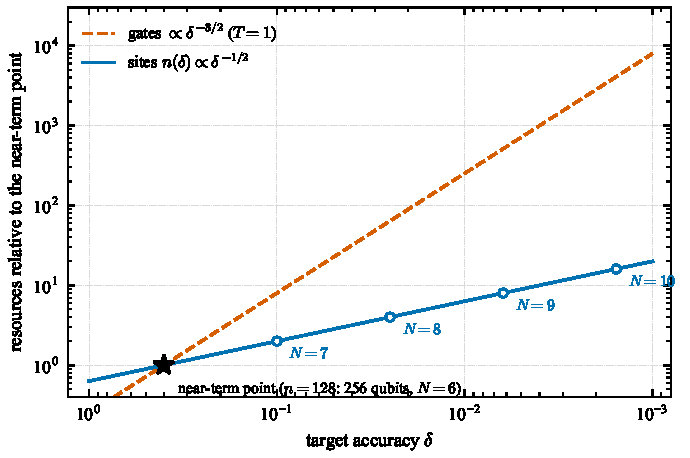
\includegraphics{figure11.pdf}
\caption{\rev{Resource scaling of the assembled algorithm, relative to the near-term point
(star): lattice sites $n(\delta)=n_{0}\,(\delta_{0}/\delta)^{1/2}\approx 81\,\delta^{-1/2}$
(solid; dyadic sizes $n=2^{N+1}$ marked) and total gate count $\propto\delta^{-3/2}$ at
$T=1$ (dashed), Eq.~\eqref{eq:finalcost}. Calibration: the one-particle D$10$ bound at
observation scale $M=3$ reaches $\delta_{0}\approx0.4$ at $N=6$ ($n_{0}=128$ sites, $256$
qubits), cf.\ Fig.~\ref{fig:waveleterrorM}.}}
\label{fig:resources}
\end{center}
\end{figure}

\medskip\noindent Every primitive invoked above
(Verstraete--Cirac--Latorre Gaussian state preparation, product-formula simulation,
phase estimation) is standard and is used as a black box; the content of this
section is the explicit ground-state circuit~\eqref{eq:gsfactor} and the assembly of
the four steps into the reconciled cost~\eqref{eq:finalcost} and qubit count.


\endgroup% --- end of new (blue) Tier-B section ---

\section{Numerical convergence data}\label{sec:numerics-figs}

\begin{figure}[h]
	\begin{center}
	
\includegraphics{figure3.pdf}
%	\begin{tikzpicture}
%	\draw (0,0) node{\includegraphics[width=0.9\textwidth]{plots/new/error_M345_k0.pdf}};
%	\draw (4.25,-3.15) node{\textbf{N}};
%	\draw (-6.35,3.6) node{$\mathbf{L}^{2}$-\textbf{error}};
%	\end{tikzpicture}
	\caption{Upper bound to the $L^{2}$-norm error between the conformal Hamiltonian $L_{0}$ and its KS approximant $L^{(N)}_{0}$ at $c=0$ on one-particle states corresponding to the subspace of the CFT Hilbert space representing wavelet details (for Daubechies wavelets D$K$) up to the \rev{observation} scale $M$ as a function of the UV cutoff scale $N$. For further details, see \cite{osborneConformal2021}.}\label{fig:waveleterrorM}
	\end{center}
\end{figure}

\begin{figure}[h]
	\begin{center}
	
\includegraphics{figure4.pdf}
%	\begin{tikzpicture}
%	\draw (0,0) node{\includegraphics[width=0.9\textwidth]{plots/new/error_M3_k0.pdf}};
%	\draw (4.15,-3.1) node{\textbf{N}};
%	\draw (-6.3,3.55) node{$\mathbf{L}^{2}$-\textbf{error}};
%	\end{tikzpicture}
	\caption{Various upper bounds to the $L^{2}$-norm error between the conformal Hamiltonian $L_{0}$ and its KS approximant $L^{(N)}_{0}$ at $c=0$ on one-particle states corresponding to the subspace of the CFT Hilbert space representing wavelet details (for Daubechies wavelets D$K$) up to the \rev{observation} scale $M$ as a function of the UV cutoff scale $N$. The parameter \rev{$s$ (labeled $\delta$ in the legend)} is related to a factorized upper bound containing an \rev{$H^{s}$}-Sobolev norm of the Daubechies D$K$ scaling function. \rev{There is deliberately no $s=2$, $K=8$ curve: that bound contains $\lVert\widehat s(\vep_{M}\,\cdot\,)\rVert_{h^{1+s}}$ with $1+s=3>\sigma_{8}=2.917$, so the quantity it plots is infinite and any value shown for it would be an artefact of the momentum truncation. This is the $3$-regularity threshold $K\ge9$ quoted above, made visible.} For further details, see \cite{osborneConformal2021}.}\label{fig:waveleterrork}
	\end{center}
\end{figure}

\begin{figure}[h]
	\begin{center}
	
\includegraphics{figure5.pdf}
%	\begin{tikzpicture}
%	\draw (0,0) node{\includegraphics[width=0.9\textwidth]{plots/new/error_l2_mom-rg_M345.pdf}};
%	\draw (5.75,-3.55) node{\textbf{N}};
%	\draw (-6,4) node{$\mathbf{L}^{2}$-\textbf{error}};
%	\end{tikzpicture}
	\caption{Upper bound to the (diagonal) $L^{2}$-norm error between the conformal Hamiltonian $L_{0}$ and its KS approximant $L^{(N)}_{0}$ at $c=1/2,1$ on one-particle states corresponding to the subspace of the CFT Hilbert space representing momenta up to the \rev{observation} scale $M$ as a function of the UV cutoff scale $N$. For further details, see \cite{osborneConformal2021}.}\label{fig:momrgerrorM}
	\end{center}
\end{figure}

\begin{figure}[h]
	\begin{center}
	
\includegraphics{figure6.pdf}
%	\begin{tikzpicture}
%	\draw (0,0) node{\includegraphics[width=0.9\textwidth]{plots/new/error_l2_mom-rg_M3_k012.pdf}};
%	\draw (5.4,-3.4) node{\textbf{N}};
%	\draw (-6,3.85) node{$\mathbf{L}^{2}$-\textbf{error}};
%	\end{tikzpicture}
	\caption{Upper bound to the (diagonal) $L^{2}$-norm error between the Virasoro generators $L_{k}$ and their KS approximants $L^{(N)}_{k}$ on one-particle states corresponding to the subspace of the CFT Hilbert space representing momenta up to the \rev{observation} scale $M$ as a function of the UV cutoff scale $N$. For further details, see \cite{osborneConformal2021}.}\label{fig:momrgerrork}
	\end{center}
\end{figure}

\begin{figure}[h]
	\begin{center}
	
\includegraphics{figure7.pdf}
%	\begin{tikzpicture}
%	\draw (0,0) node{\includegraphics[width=0.9\textwidth]{plots/new/error_hs_mom-rg_M3_k234.pdf}};
%	\draw (5.7,-3.5) node{\textbf{N}};
%	\draw (-6,3.95) node{$\mathbf{HS}$-\textbf{error}};
%	\end{tikzpicture}
	\caption{Upper bound to the (off-diagonal) Hilbert-Schmidt (HS)-norm error between the Virasoro generators $L_{k}$ and their KS approximants $L^{(N)}_{k}$ on one-particle states corresponding to the subspace of the CFT Hilbert space representing momenta up to the \rev{observation} scale $M$ as a function of the UV cutoff scale $N$. Note that this error vanishes for the generators of the M\"obius group, $k=0,\pm 1$. For further details, see \cite{osborneConformal2021}.}\label{fig:momrgerrorHS}
	\end{center}
\end{figure}

\begingroup% --- resubmission: new correlator-level convergence figure ---
\begin{figure}[h]
	\begin{center}
	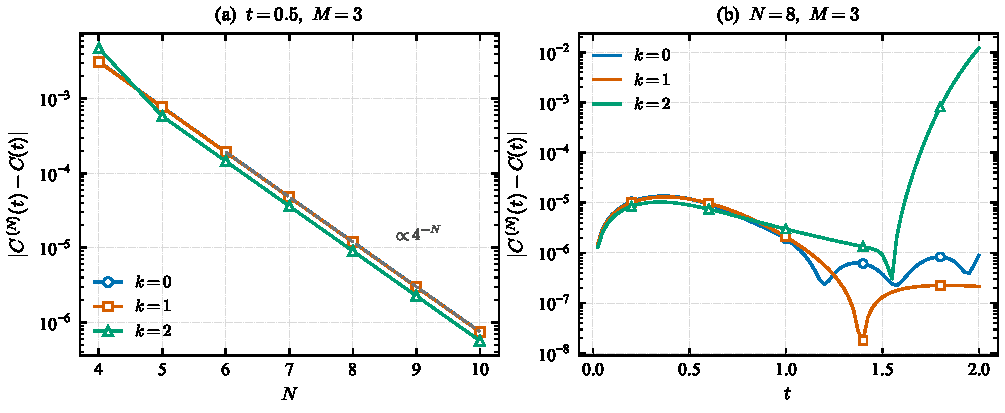
\includegraphics[width=\textwidth]{figure10.pdf}
	\caption{\rev{Correlator-level convergence of the simulated dynamics (momentum-cutoff RG,
	chiral fermion; the one-particle inputs are shown in
	Figs.~\ref{fig:momrgerrorM}--\ref{fig:momrgerrorHS}). Plotted is the error
	$|C^{(N)}(t)-C(t)|$ of the two-point function
	$C^{(N)}(t)=\langle\Omega_N|\,a^{\dagger}(f)\,a_t(g)\,|\Omega_N\rangle$ of bounded
	smeared fields localized at observation scale $M=3$, with
	$a_t(g)=e^{itH_k^{(N)}}a(g)e^{-itH_k^{(N)}}$, $H_k^{(N)}=L_k^{(N)}+L_{-k}^{(N)}$,
	evaluated against a continuum reference (momentum cutoff $2^{11}$). (a)~At fixed
	$t=0.5$ the error decays as $4^{-N}=2^{-2N}$ for $k=0,1,2$ (fitted per-step ratio
	$4.00$; dashed guide; the $k=0$ and $k=1$ curves nearly coincide), realizing the
	$\varepsilon_{N}^{2}$ rate of Theorem~S1(ii) at the level of dynamical correlation functions. (b)~At
	fixed $N=8$ the error oscillates beneath a bounded envelope for $k=0,1$, whereas for
	$k=2$ it grows sharply once the evolved energy shell $e^{c_k t}$ of Lemma~S5
	reaches the lattice cutoff (here $t\gtrsim1.5$) --- the shell-confinement mechanism
	made visible. The times are quoted in the normalisation $\vep_{N}=2^{-N}$ of the script
	that produces this figure rather than the $\vep_{N}=L2^{-N}$ of the text; what is claimed
	here is the $4^{-N}$ rate and the qualitative envelope, neither of which depends on that
	choice.}}\label{fig:corrconv}
	\end{center}
\end{figure}
\endgroup

\end{document}